\section{ネットワークの変更}
春山らの先行研究では,\figref{fig:haruyama_net}に示すネットワークを使用していた.
一方でfelipeらの先行研究によると,コマンドによってモデルを分岐する形式のネットワークがより経路追従の成功率が向上すると報告している.
そのため,今回の研究ではfelipeらによって提案されたネットワークを参考に\figref{fig:branched}に示す,新たなネットワークを構築した.
ネットワークの入力は春山らが作成したものと同様で,64×48 の RGB画像と\tabref{tab:cmd_dir}に示す,目標方向のワンホットベクトルで,出力はヨー方向の角速度である.
また,損失関数や活性化関数などのパラメータは春山らの手法と同様である.

\begin{figure}[htbp]
  \centering
  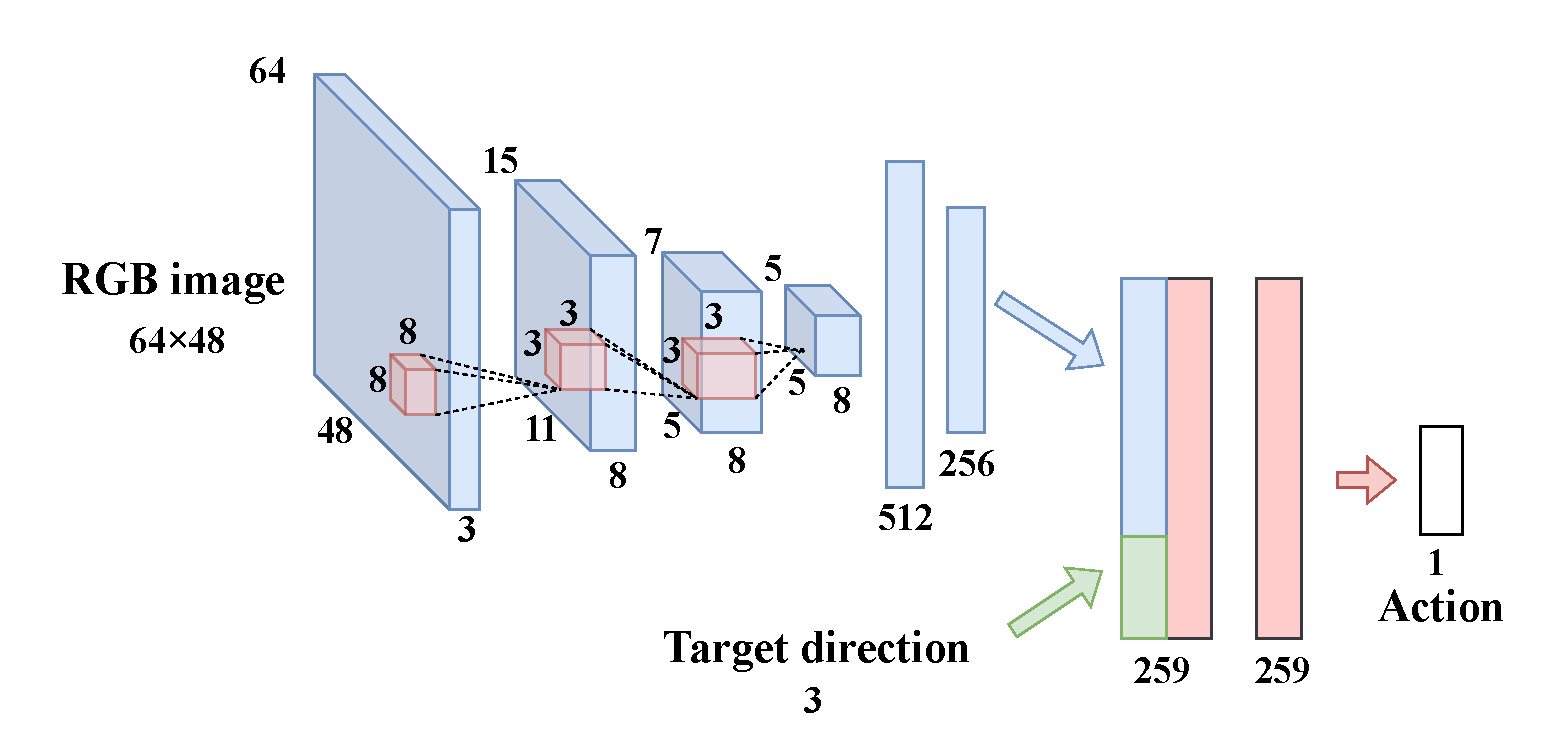
\includegraphics[width=110mm]{images/pdf/haruyama/net.pdf}
  \caption[Structure of the network haruyama and others used]{Structure of the network haruyama and others used(Quoted from \cite{fujiwara2023})}
  \label{fig:haruyama_net}
\end{figure}

\begin{figure}[htbp]
  \centering
   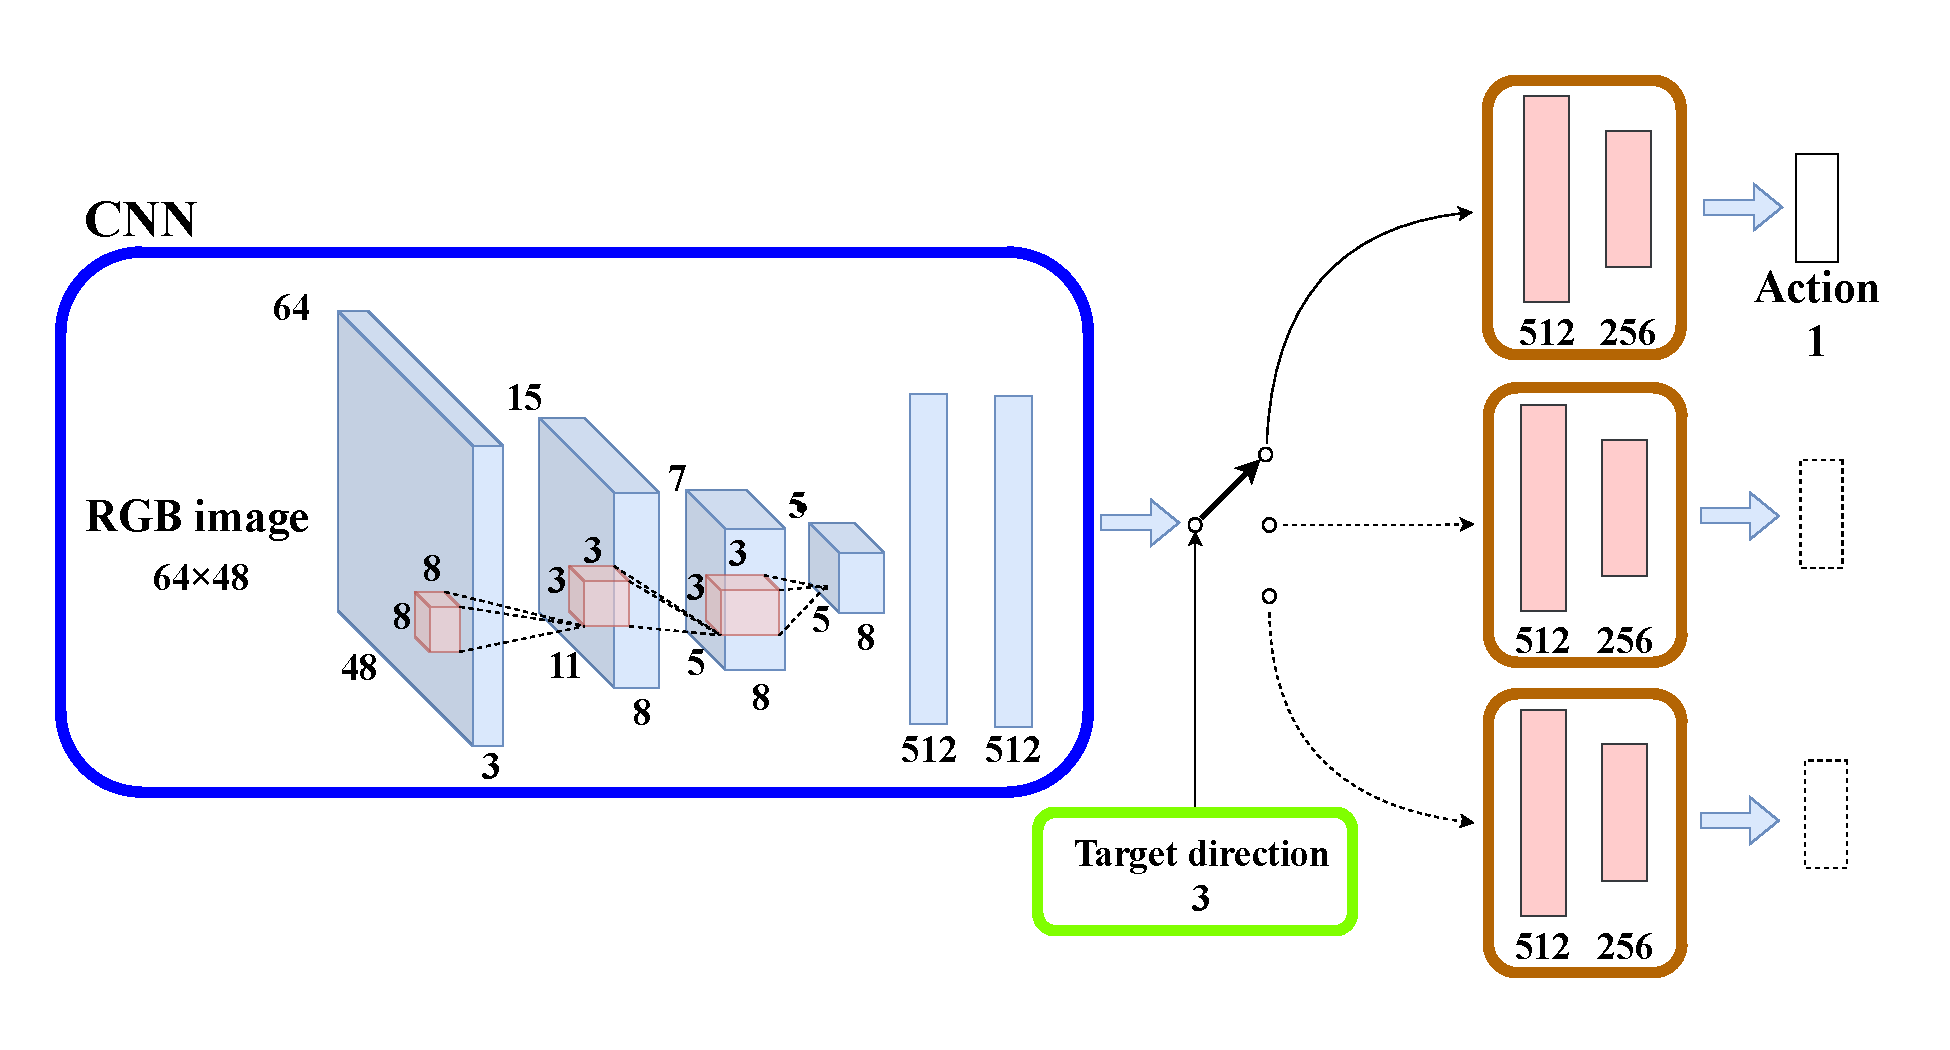
\includegraphics[width=110mm]{images/pdf/ishiguro/branched.pdf}
   \caption{Branched network}
   \label{fig:branched}
\end{figure}

\begin{table}[htbp]
  \centering
  \caption{Target direction and data for path-following module}\label{tab:cmd_dir}
  \begin{tabular}{|c|c|}
  \hline
  Target direction & Data        \\
  \hline
  Go straight   & {[}1,0,0{]} \\
  Turn left   & {[}0,1,0{]} \\
  Turn right   & {[}0,0,1{]} \\
  Stop   & {[}0,0,0{]}\\
  \hline
  \end{tabular}
\end{table}

\clearpage